% -*- coding: utf-8 -*-
% !TEX program = xelatex
\documentclass[14pt]{jnuthesis}

\usepackage{enumerate}
\usepackage{xeCJK}
\usepackage[numbers,sort&compress]{natbib}
\usepackage{algorithm}
\usepackage{algorithmicx}
\usepackage{algpseudocode}
\usepackage{bm}

\begin{document}

\renewcommand{\title}{The English title} % 一般格式为:A YYY based on XXX
\renewcommand{\biaoti}{中文标题} % 一般格式为:基于 XXX 的 YYY
\renewcommand{\xueyuan}{网络空间安全学院}
\renewcommand{\zhuanye}{网络空间安全}
\renewcommand{\xingming}{学生姓名} % 如果遇到打不出的字请用 {\CJKfontspec{宋体}字},例如\renewcommand{\xingming}{字{\CJKfontspec{宋体}字}字}
\renewcommand{\xuehao}{2019999999}
\renewcommand{\daoshi}{指导老师姓名}

\newcommand{\upcite}[1]{\textsuperscript{\cite{#1}}}
\newcommand{\upupcite}[1]{\textsuperscript{\textsuperscript{\cite{#1}}}}

\titlepage

\pagenumbering{Roman} % 绪论前为罗马数字页码

\addcontentsline{toc}{chapter}{\hspace{-1em}诚信声明}

\statement

\begin{zhabstract}

\addcontentsline{toc}{chapter}{\hspace{-1em}摘要}

\zhaiyao
摘要应扼要叙述本论文的主要内容、特点,文字要精炼,是一篇具有独立性和完整性的短文,应包括本论文的主要成果和结论性意见。摘要一般独立一段,不宜使用公式、图表等非常规文本类型,不标注引用文献编号,避免将摘要写成目录式的内容介绍,也不要将摘要写成“前言”。编写摘要应注意:客观反映原文内容,不得简单地重复题名中已有的信息,要着重反映论文的新内容和特别强调的观点,直观给出量化的(对比)结果。摘要在总结前人工作时宜采用第三人称过去式的写法 (如“对……进行了研究”,“综述了……”等)。摘要以 300-400 字左右为宜,可在写完初稿时再写摘要。请注意,使用 XeLaTeX 进行编译,通常一次编译需要使用 XeLaTeX 编译至少两次(使用 BibTeX 请参阅参考文献)。

\guanjianci
关键词 1;关键词 2;关键词 3;关键词 4;关键词 5

\end{zhabstract}

\begin{enabstract}

\addcontentsline{toc}{chapter}{\hspace{-1em}Abstract}

\abstract
This is an abstract. 

\keywords
Keyword 1; Keyword 2; Keyword 3; Keyword 4; Keyword 5

\end{enabstract}

\pagenumbering{arabic}

\tableofcontents

\chapter{绪论}\setcounter{page}{1} % 此处修正绪论部分页码为 1。模板仅供参考,请根据自己实际情况进行调整。
\label{chap:1}

一段总结性文字,讲述该章节的各节内容,除结论章节以后每一章节同。

\section{研究背景}

正文部分回车时应当使用两个回车而不是两个反斜杠。

例如,这样。

\section{研究意义}

文字。

文字。

\section{本文的主要工作}

% 模板仅供参考,请根据自己实际情况进行调整。

为了解决什么问题,本文怎么样。为了更好地进行描述,本文的创新点有如下三点:

\begin{enumerate}[1)]
	\item 创新点 1。解释创新点 1。
	\item 创新点 2。解释创新点 2。
	\item 创新点 3。解释创新点 3。
\end{enumerate}

\section{本文的组织结构}

为了更好地阐述本文的工作,本文的结构如下。第~\ref{chap:1}~章节是引言,主要讲述了……第~\ref{chap:2}~章节是……第~\ref{chap:3}~章节是……第~\ref{chap:4}~章节是……第~\ref{chap:5}~章节是……

% 模板仅供参考,请根据自己实际情况进行调整。

\section{术语说明}

科学问题(scientific problem):科学问题,指在科学研究中需要解决的问题,这些问题通常是具有创新性和挑战性的,往往是从工程实践中抽象出来的某一类共通的问题。这些问题的解决方案可以指导工程的实践过程,可以推动科学和工程的发展,以“实践 $\rightarrow$ 认知 $\rightarrow$ 实践”的方式不断提高人类对自然和社会的认识和理解。发现、提炼或制造科学问题,是“提出问题 $\rightarrow$ 分析问题 $\rightarrow$ 解决问题”中最重要的一环。

可编程的(programmable):某计算机系统、设备或器件等是可编程的意味着其具有可编程性,即可以通过编程或配置来实现不同的功能或行为。可编程性是现代计算机技术的重要特征之一,它可以使计算机系统或设备具有更高的灵活性、可定制性和可扩展性。

鲁棒性(robustness):鲁棒性是指系统或算法对于意外情况或异类输入的处理能力,例如能够在面对异常或错误的情况下保持稳定性和正确性的能力。

傅里叶变换(Fourier transform,简称 FT):傅里叶变换是一种数学工具,常用于将一个函数表示为一组正弦或余弦函数的和。

% 模板仅供参考,请根据自己实际情况进行调整。一般只在第一次出现专业名词或中文有多种意义的词后面标英文,可附缩写,在写了缩写后,相近出现的通常采用缩写。

\chapter{非常规文本类型格式模板}
\label{chap:2}

本章节提供了非常规文本类型的格式模板及其引用。

\section{图}

本节介绍了图。

\subsection{图}

图~\ref{fig:development}~是……

\begin{figure*}[htbp] % 没有多栏,暂不考虑跨栏问题
	\centerline{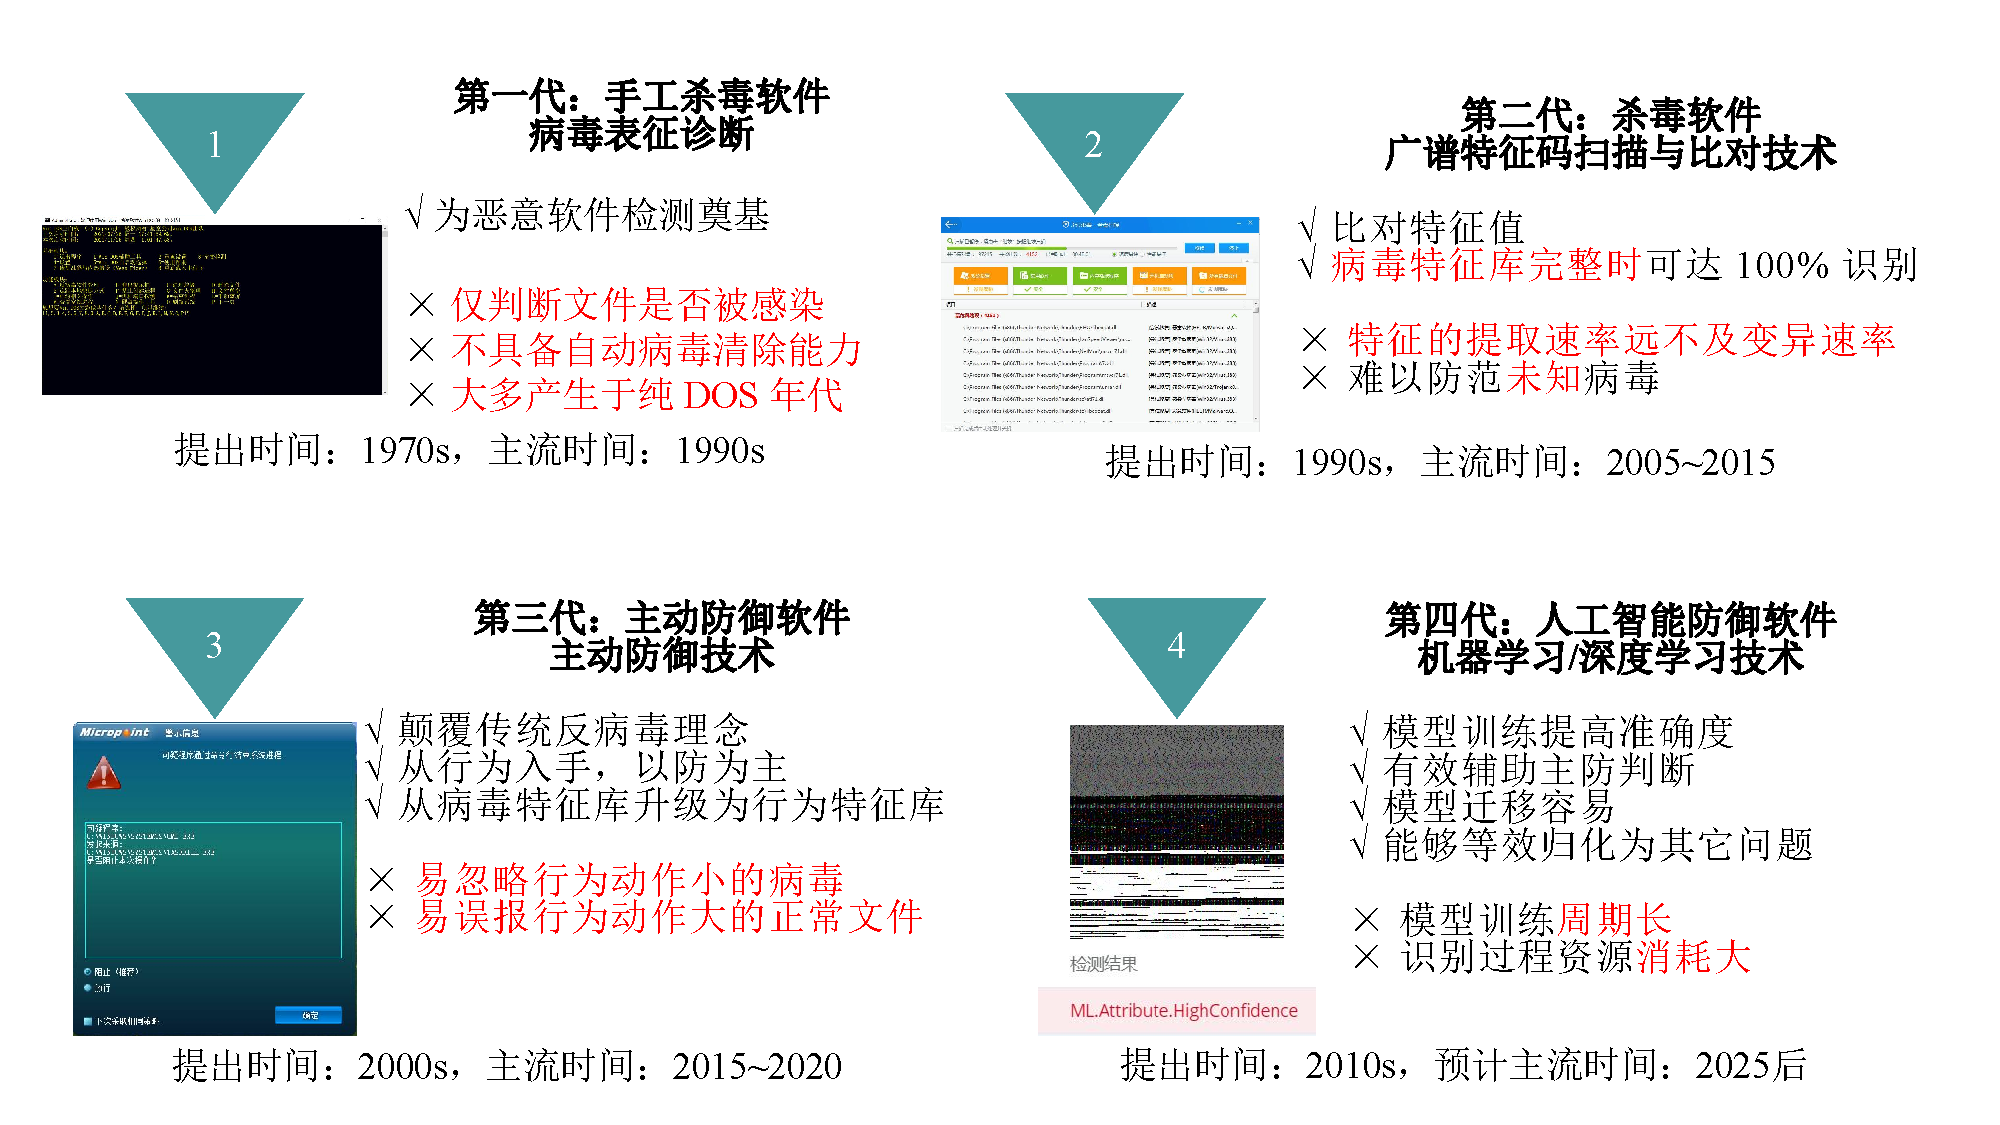
\includegraphics[width=0.95\textwidth]{figs/development.pdf}} % 建议用一个文件夹 fig 放置图片
	\caption{XXX} % caption 在图后面
	\label{fig:development} % 一般图的 label 是 {fig:XXX}
\end{figure*}

\subsection{子图}

图~\ref{fig:trend}~是……其中(a)……

\begin{figure*}[htbp]
	\centering
	\begin{tabular}{cc}
		\centerline{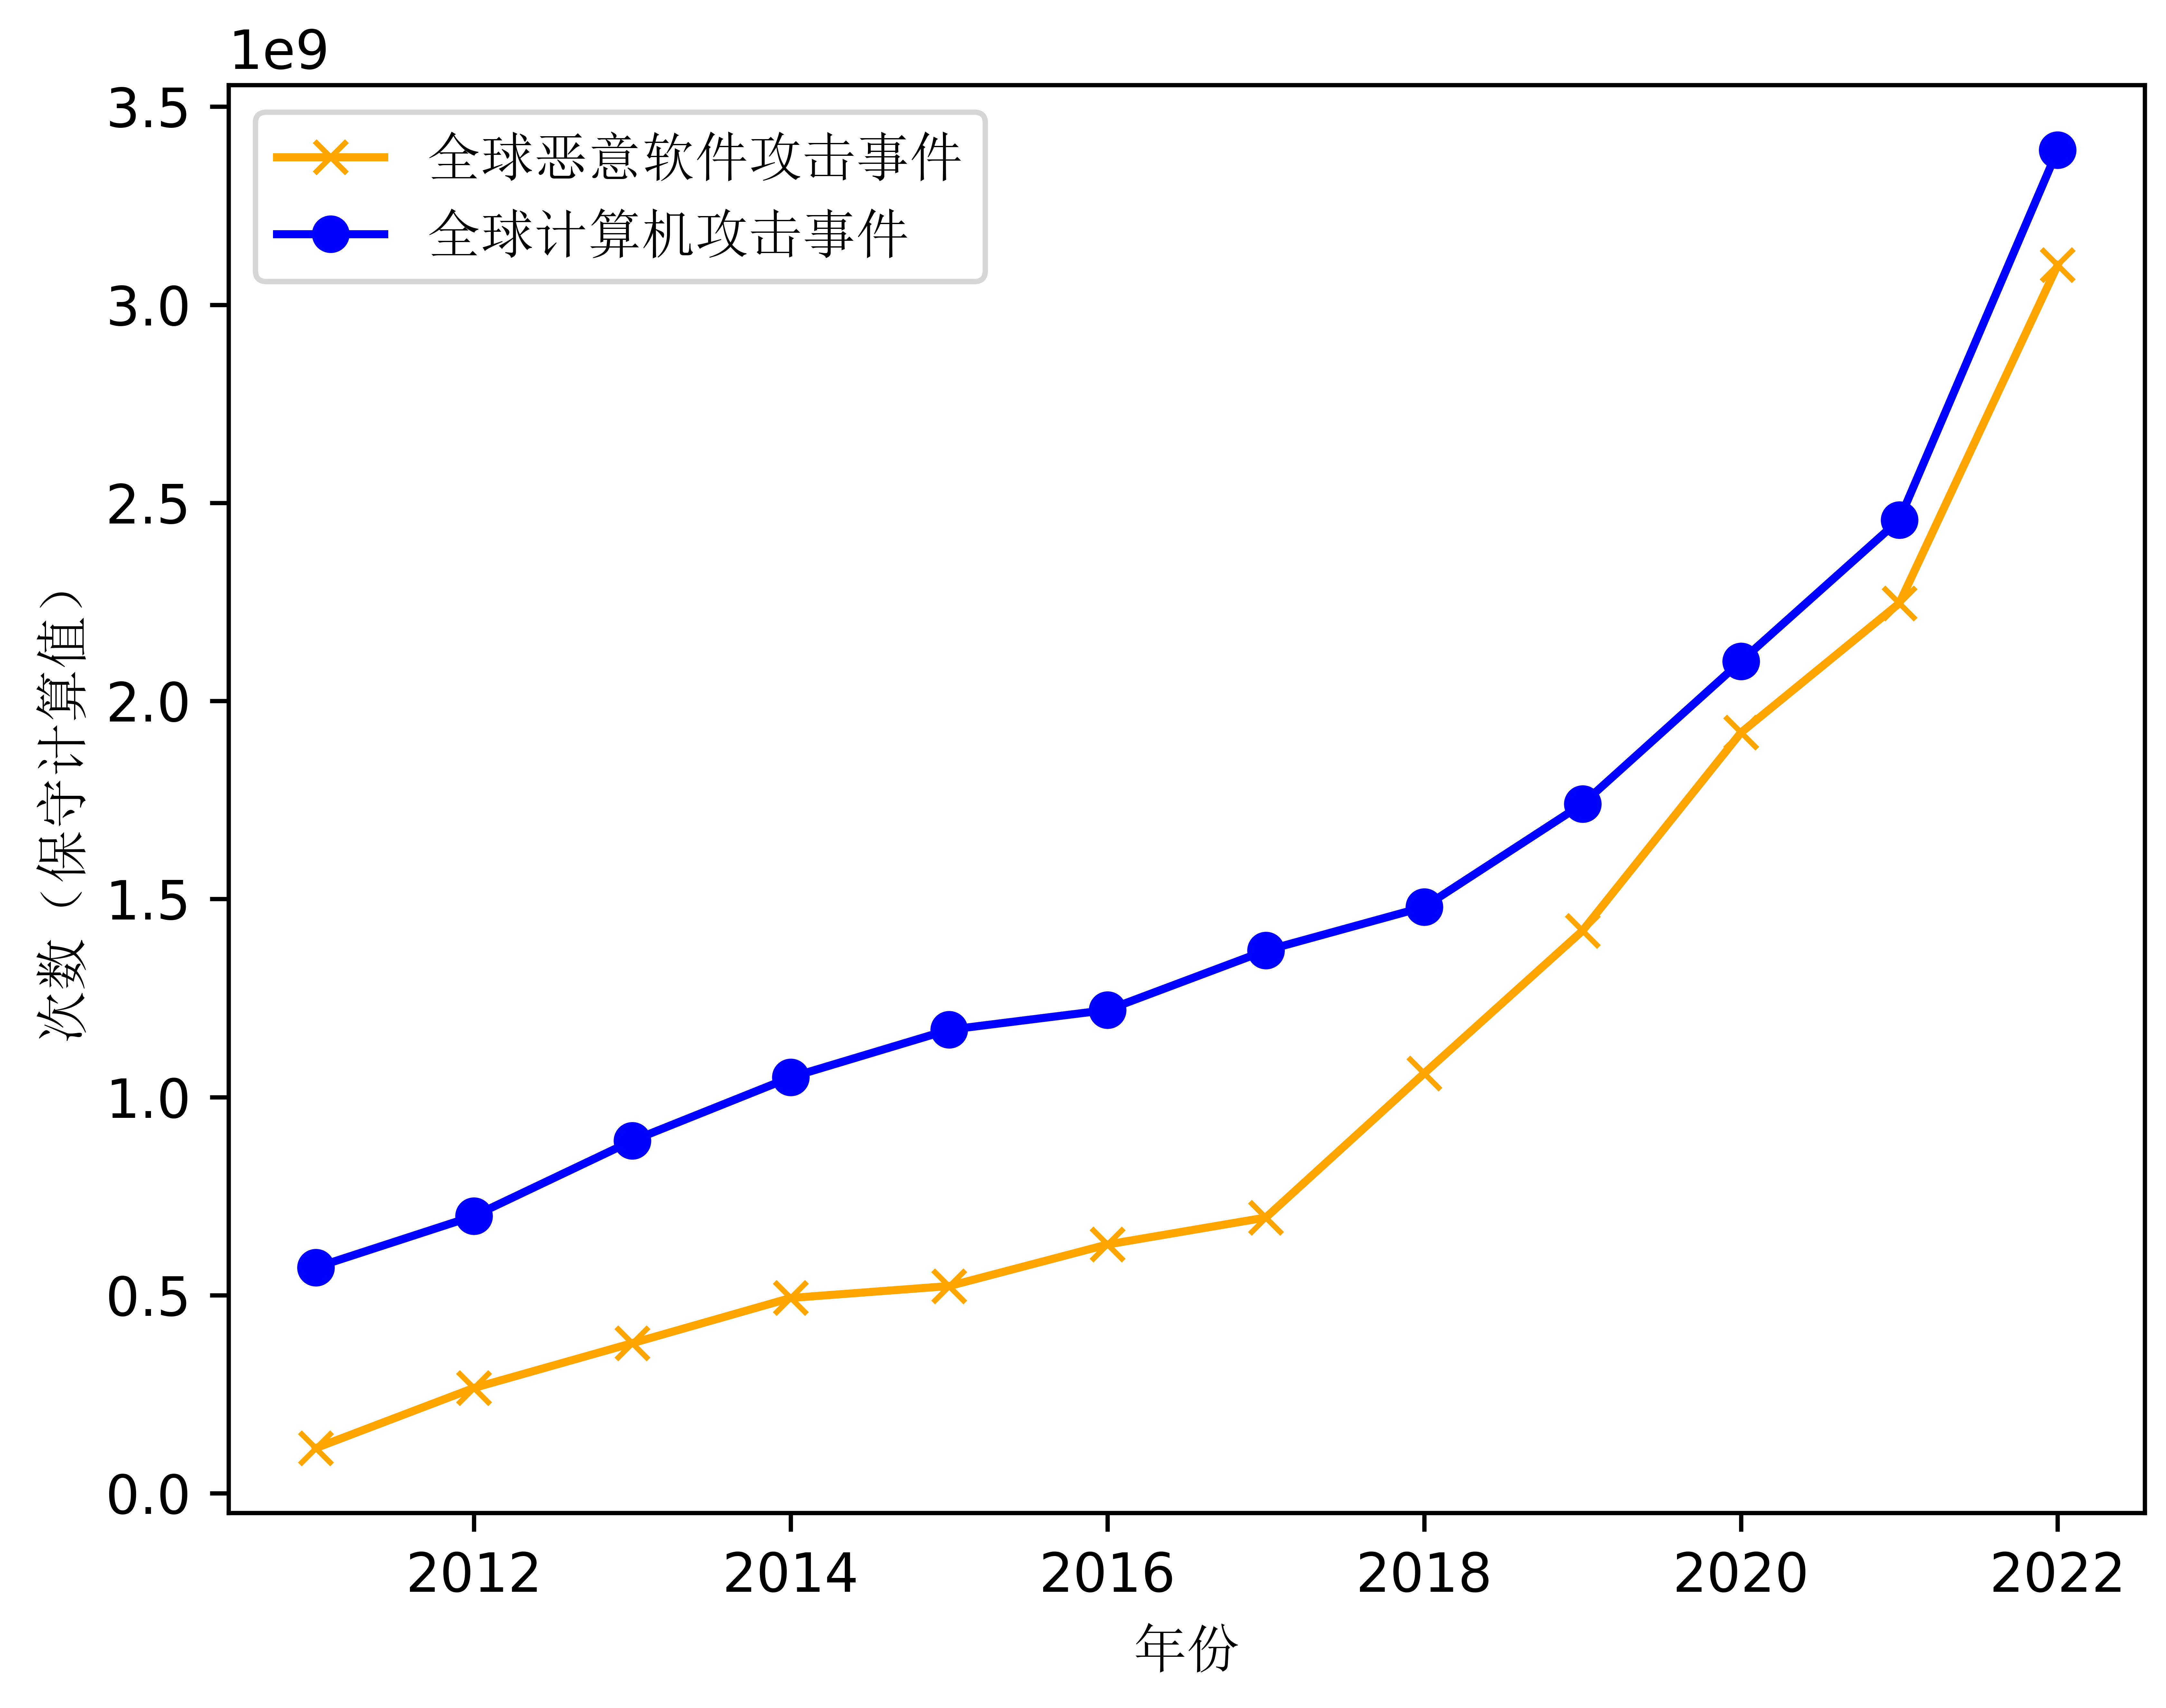
\includegraphics[width=0.4\textwidth]{figs/trends/trend_a.png}} & 
		\centerline{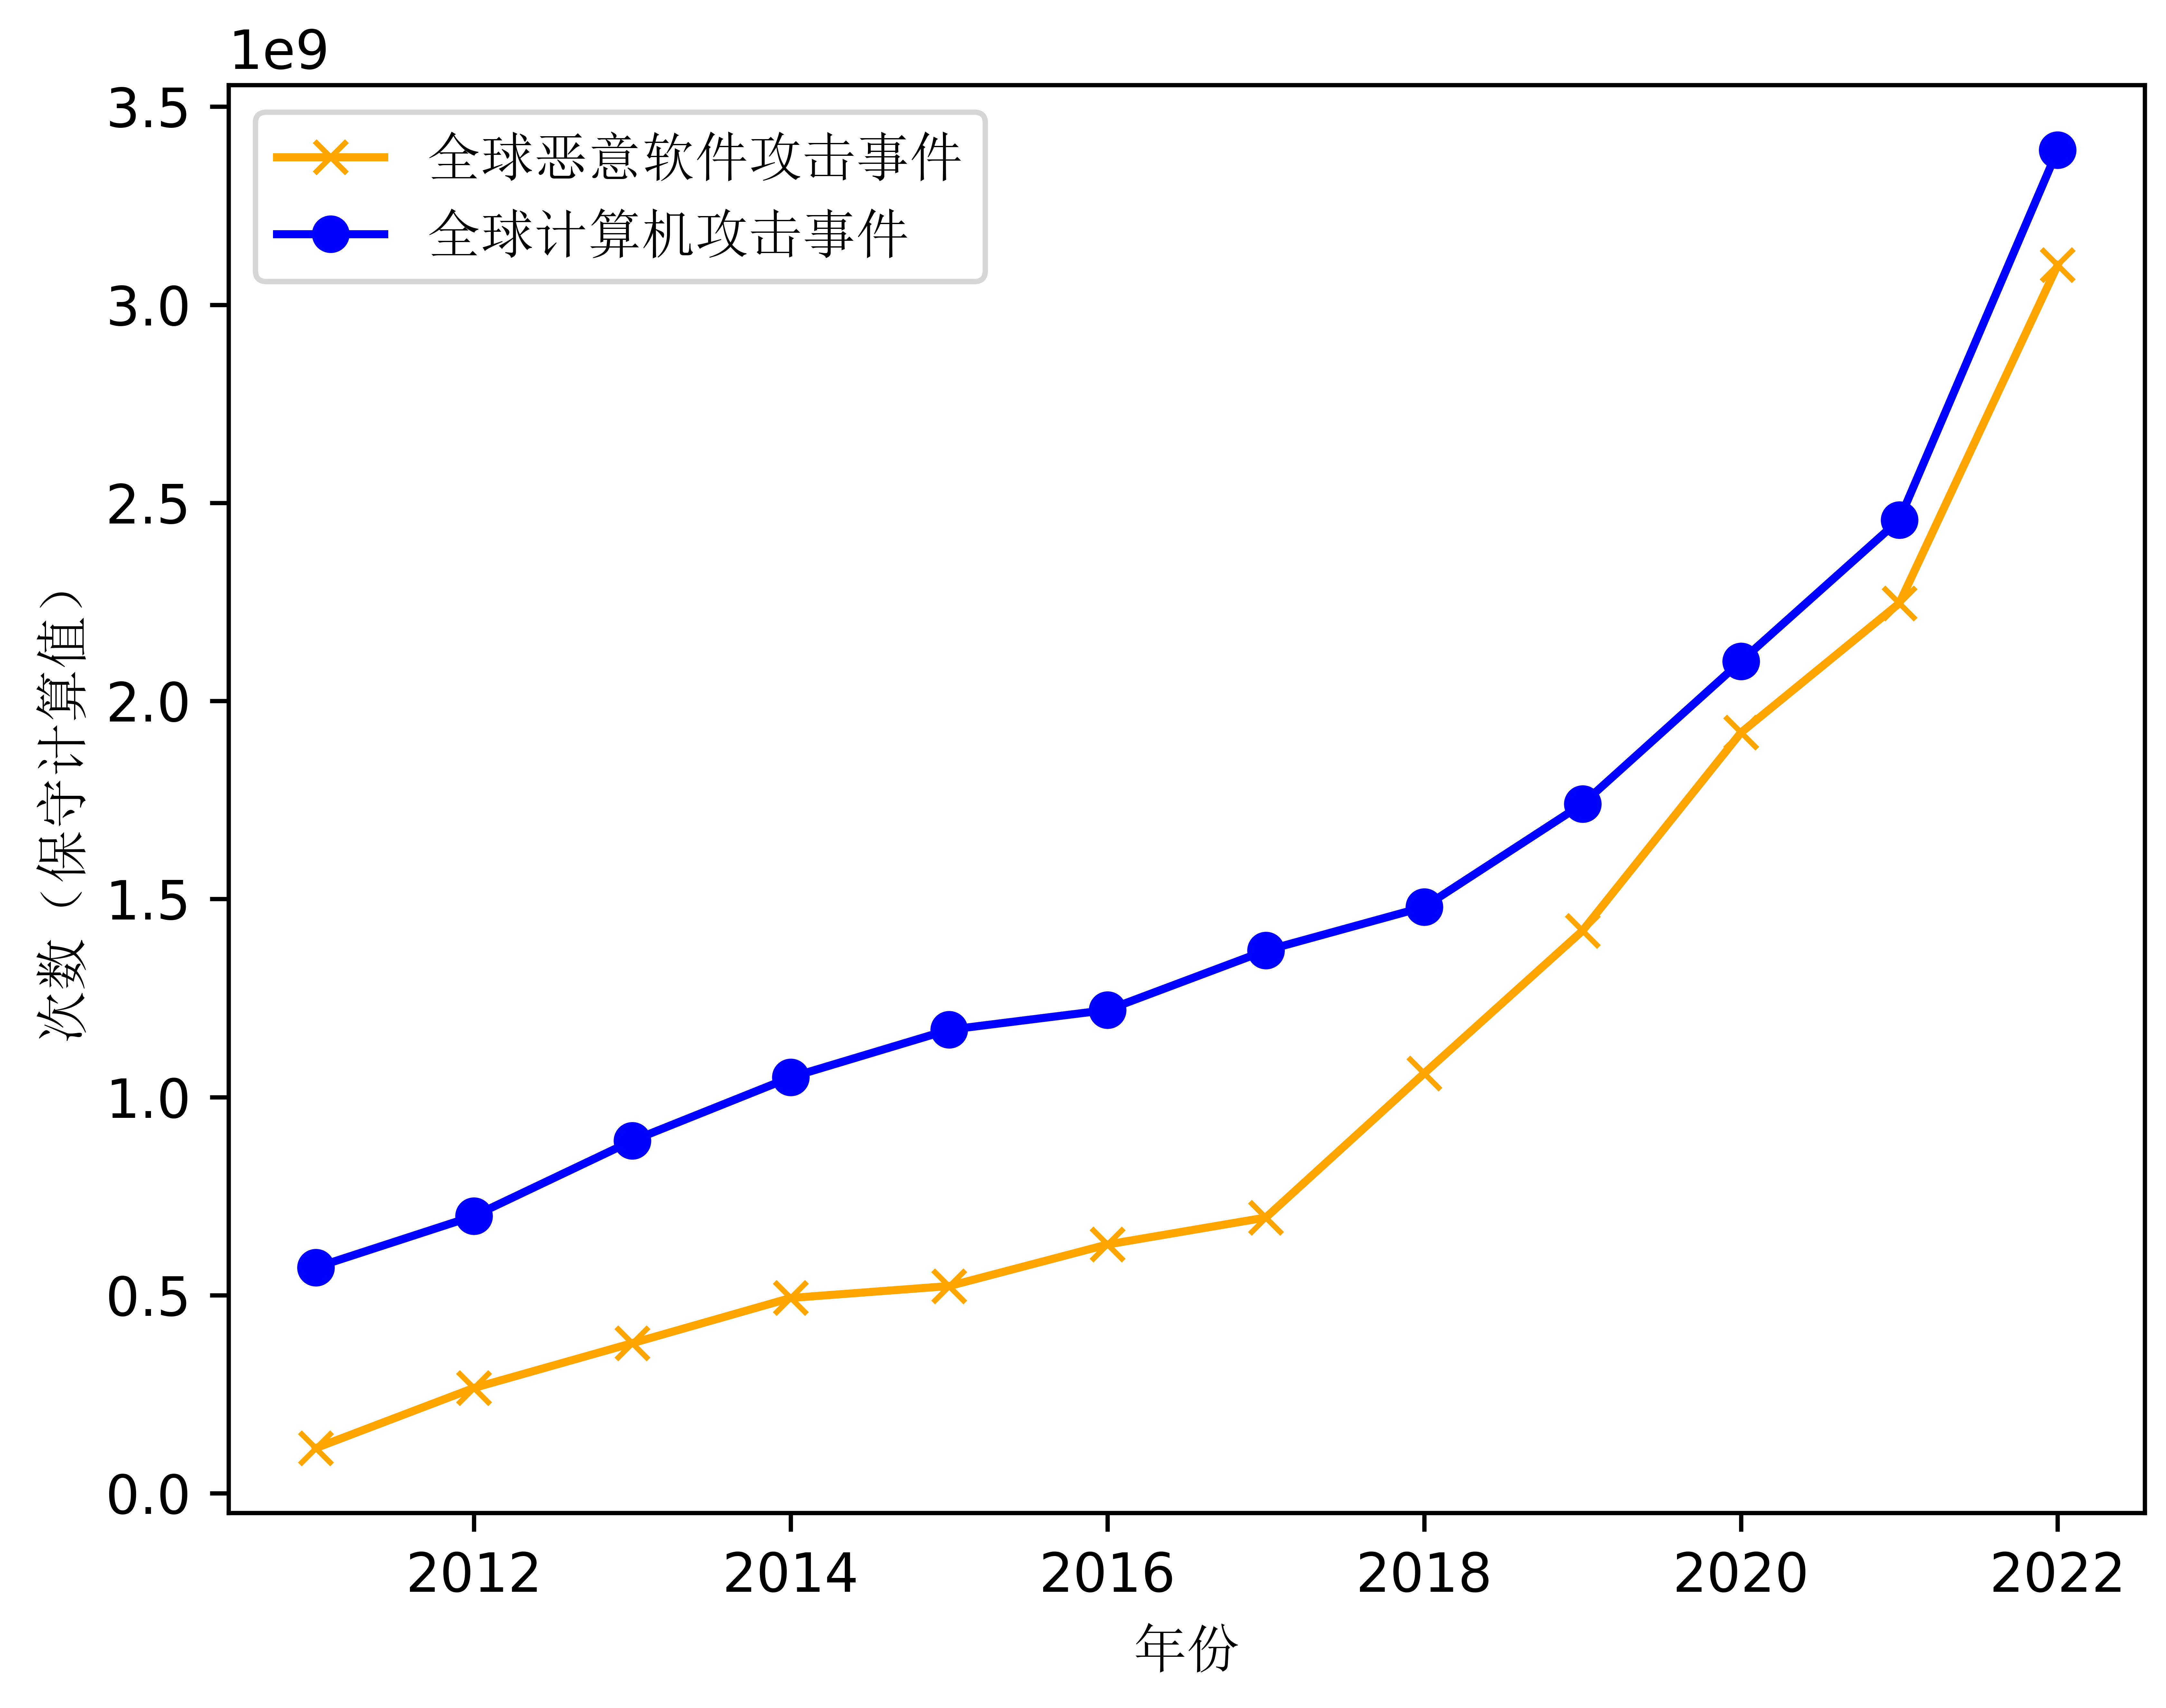
\includegraphics[width=0.4\textwidth]{figs/trends/trend_b.png}}  \\
		\centerline{(a)} & \centerline{(b)}  \\
		\centerline{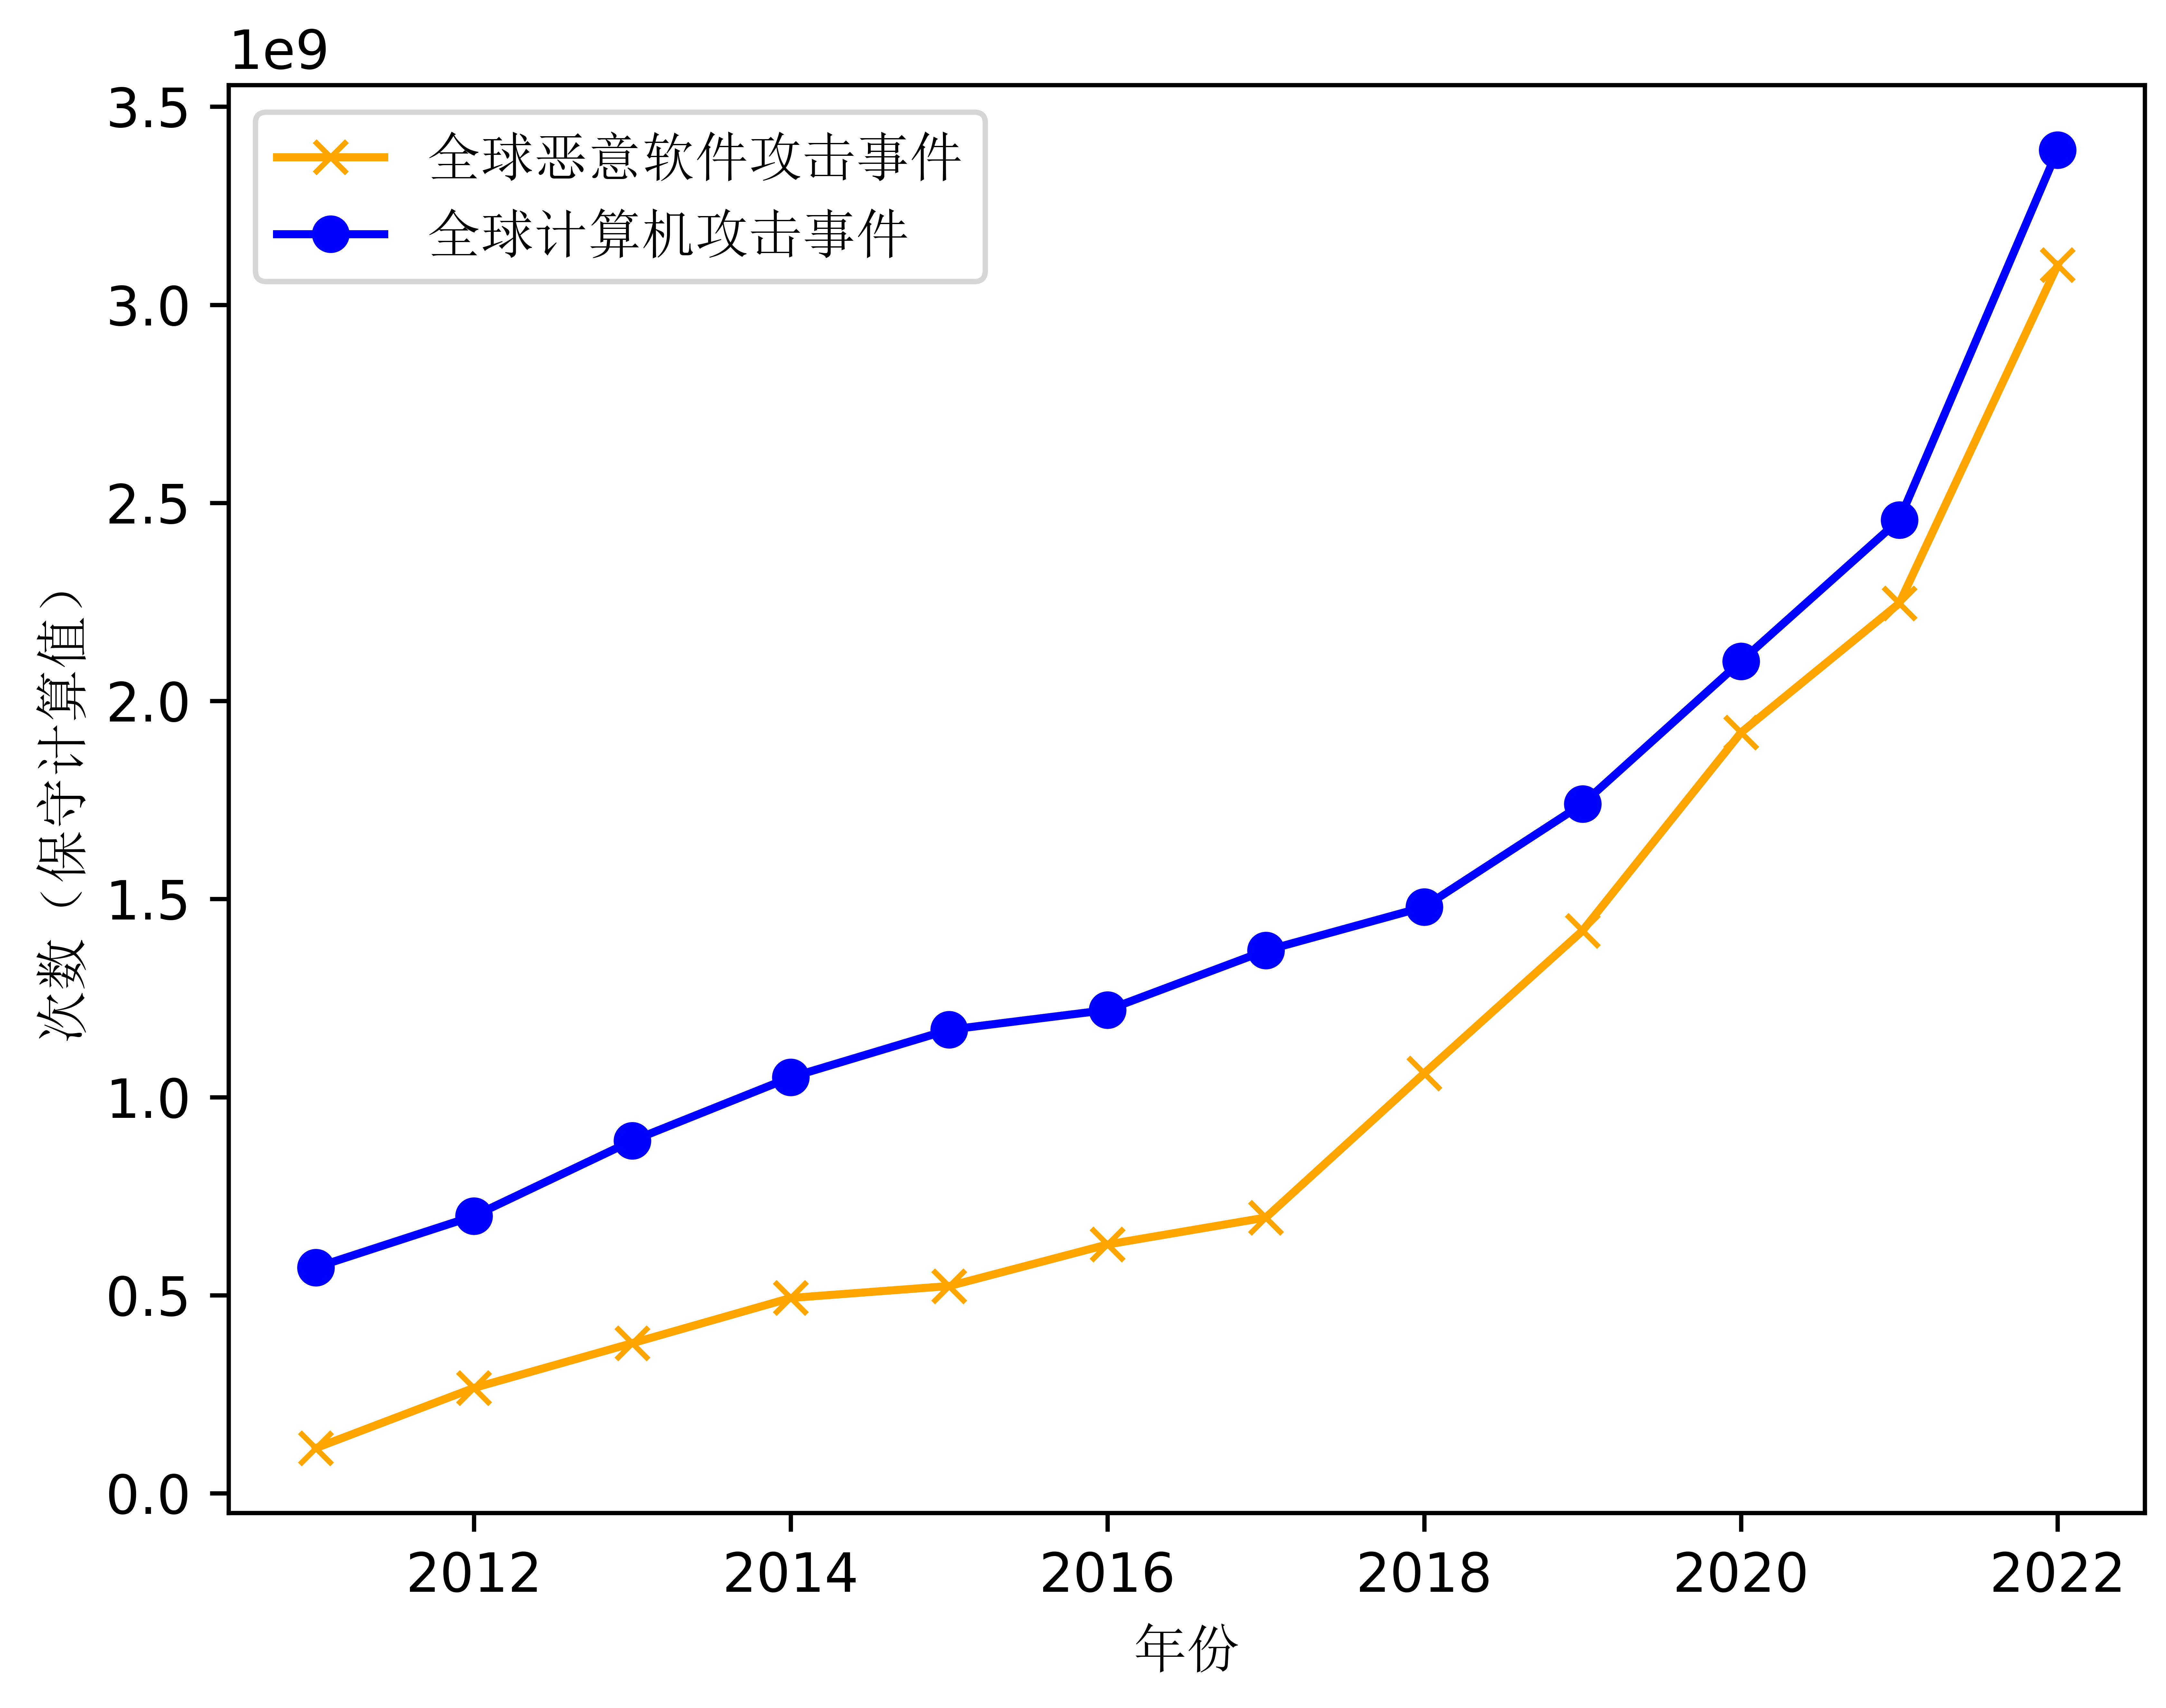
\includegraphics[width=0.4\textwidth]{figs/trends/trend_c.png}} & 
		\centerline{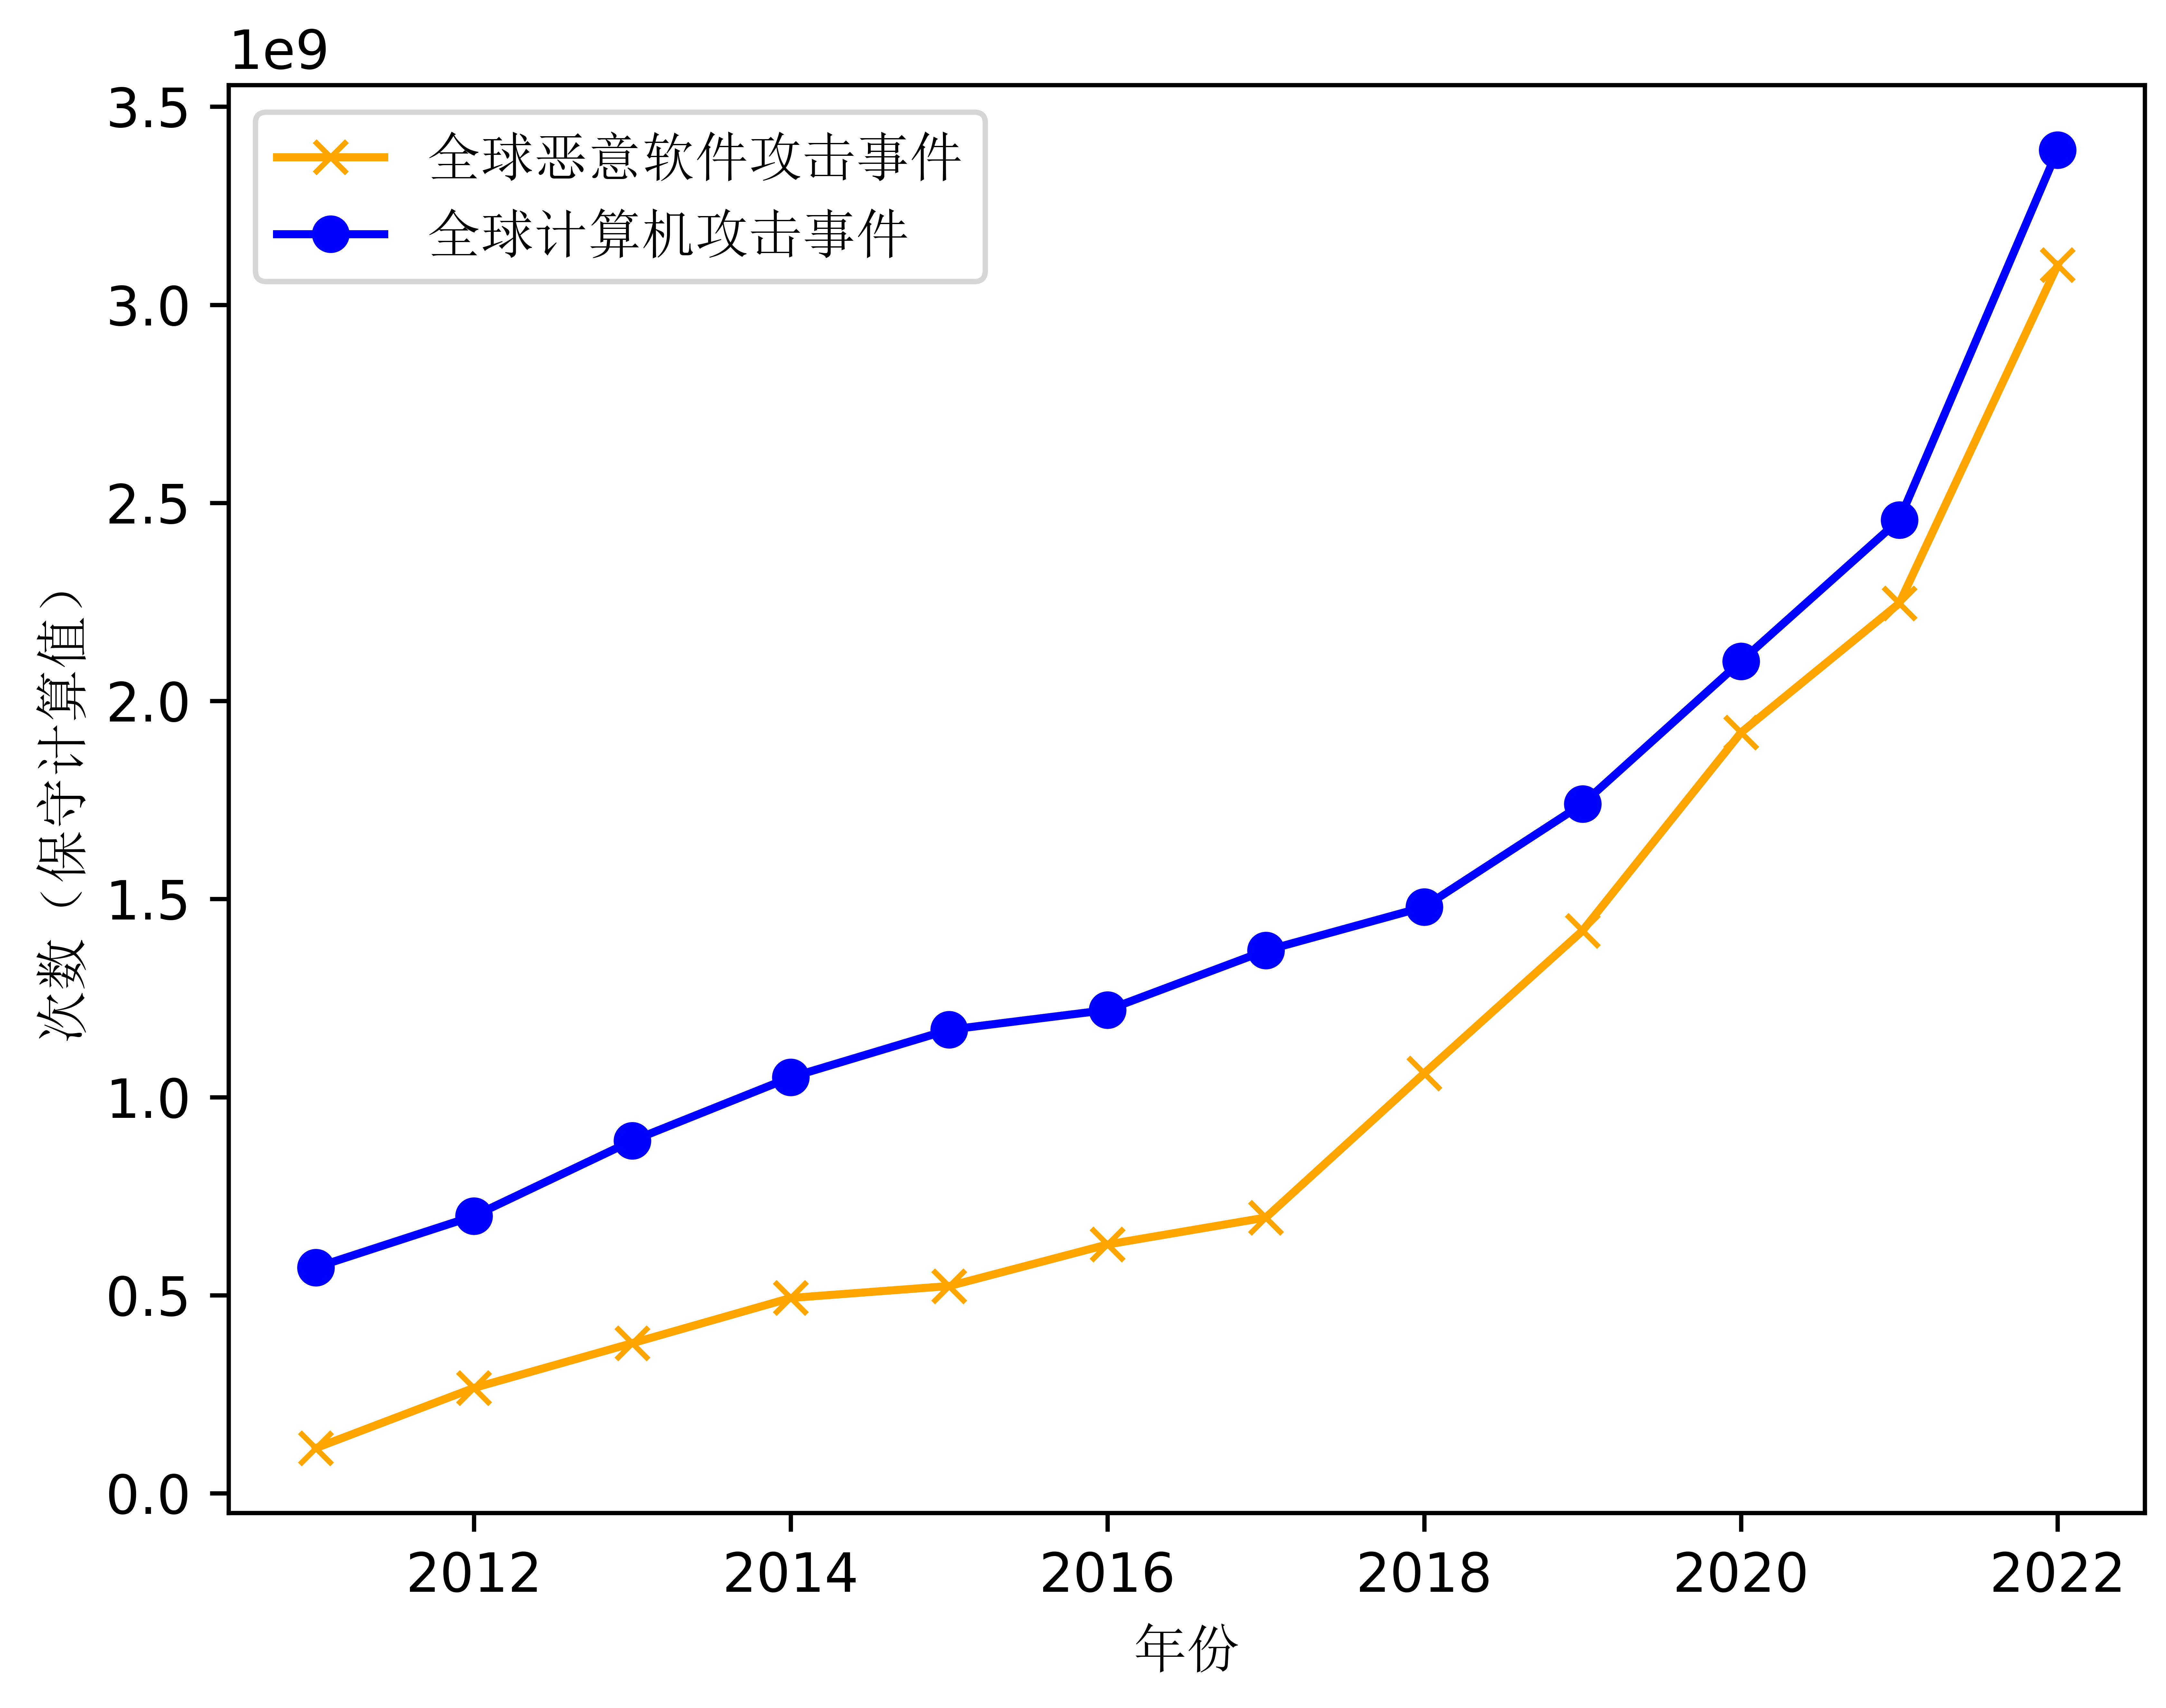
\includegraphics[width=0.4\textwidth]{figs/trends/trend_d.png}}  \\
		\centerline{(c)} & \centerline{(d)}  \\
	\end{tabular}
	\caption{XXX} % caption 在图后面
	\label{fig:trend} % 一般图的 label 是 {fig:XXX}
\end{figure*}

\section{表}

表,一般用三线表。

表~\ref{tab:compare}~真美好,表~\ref{tab:complex}~真复杂。

\begin{table}[htbp]
	\caption{XXX}
	\centering % \tiny\centering 可缩小字体
	\begin{tabular}{cccc}
		\hline
		\textbf{项目} & \textbf{表头 1} & \textbf{表头 2} & \textbf{表头 3}  \\
		\hline
		AAA & \textbf{100.00\%} & 99.00\% & 98.00\%  \\
		BBB & 99.00\% & 98.00\% & 97.00\%  \\
		\textbf{CCC} & 99.00\% & \textbf{100.00\%} & \textbf{99.00\%}  \\
		\hline
	\end{tabular}
	\label{tab:compare}
\end{table}

\begin{table}[htbp]
	\caption{主流的不良言论识别方案}
	\centering
	\begin{tabular}{m{1cm}m{4.1cm}m{4.4cm}m{4.3cm}}
		\hline
		 & \textbf{传统计量方法} & \textbf{词典法} & \textbf{自然语言处理法}\upcite{b3-2-3-2}  \\
		\hline
		方法 & 通过人工标注识别并编制成指数进行计算 & 利用词典进行无监督学习计算文本相似度进而分析文本的表意倾向 & 利用 transformer 超强的特征抽取能力来学习词语的双向编码  \\
		 &  &  &  \\
		优点 & 统计学原理;解释性强 & 无监督学习;解释性强;灵活度高 & 融合了上下文信息,能自动进行决策  \\
		 &  &  &  \\
		缺点 & 主观性较强;处理的数据量有限 & 易忽略上下文否定词 & 解释性差;黑盒模型;训练模型耗能大、耗时长  \\
		\hline
	\end{tabular}
	\label{tab:complex}
\end{table}

\section{伪代码}

事实上,伪代码在 WPS 文字或 word 中可以被认为是一个两行一列的三线表,在表的第二行中完成所有伪代码的书写即可。在 LaTeX 中,一个可能的伪代码如算法~\ref{alg:1}~所示。如果不希望使用伪代码,可使用流程图,即绘制 PPT 后转 PDF 使用图的方式引入 LaTeX。

\begin{algorithm}[H]
	\caption{自动调整不均匀数据集权值。}
	\begin{algorithmic}[1]
		\State \textbf{Initial } $\bm{C} \gets \{C_1, C_2, \cdots, C_n\}$ with length $n$
		\State \textbf{let } $S \gets \mathrm{sum}(\bm{C})$;
		\For {$i \gets 1 \textbf{ to } n$}
			\State $C_i \gets S / C_i;$
		\EndFor
		\State \textbf{let } $S \gets \mathrm{sum}(\bm{C})$;
		\For {$i \gets 1 \textbf{ to } n$}
			\State $C_i \gets C_i / S;$
		\EndFor
		\If {$C_0 = 1$} % 直接用等号表示比较,不需要两个等号
			\State Do something;
		\ElsIf {$C_1 \neq 0.5$}
			\State Do something;
		\ElsIf {$C_0 \leqslant 0.1$} % 可直接使用小于等于、大于等于号
			\State Do something;
		\Else
			\State Do nothing;
		\EndIf
		\State \Return $\bm{C}$ // $\bm{C}$ 即为权重因子。 
	\end{algorithmic}
	\label{alg:1}
\end{algorithm}

\section{公式}

这里是公式,一般有行内公式 $a + b \leqslant c$ 和行间公式~\eqref{eq:CEEMDAN}~两种。特殊地,有公式~\eqref{eq:SEAB}~。

\begin{equation}
	\textit{SE}(M, R) = \mathop{\lim}_{N \to \infty}\left\{-\ln\left[\cfrac{A^M(R)}{B^M(R)}\right]\right\}
	\label{eq:SE}
\end{equation}

\begin{equation}
	\begin{aligned}
		\left\{\begin{array}{r@{{}={}}l}
			A^M(R) & \cfrac{1}{N - M}\mathop{\sum}_{i = 1}^{N - M}A_i^M(R)  \\
			B^M(R) & \cfrac{1}{N - M}\mathop{\sum}_{i = 1}^{N - M}B_i^M(R)  \\
			A_i^M(R) & \cfrac{1}{N - M - 1}A_i  \\
			B_i^M(R) & \cfrac{1}{N - M - 1}B_i
		\end{array}
		\right.
	\end{aligned}
	\label{eq:SEAB}
\end{equation}

某些公式不想要标号,如:

\begin{equation*}
	\begin{aligned}
		S & = \cos<(1, 2, 2, 1, 1, 0), (2, 2, 2, 1, 1, 2)>  \\
		 & = \cfrac{1 \times 2 + 2 \times 2 + 2 \times 2 + 1 \times 1 + 1 \times 1 + 0 \times 2}{\sqrt{1^2 + 2^2 + 2^2 + 1^2 + 1^2 + 0^2}\sqrt{2^2 + 2^2 + 2^2 + 1^2 + 1^2 + 2^2}}  \\
		 & = \cfrac{12}{\sqrt{11} \times \sqrt{18}} = \cfrac{2\sqrt{22}}{11} \approx 85.28\%
	\end{aligned}
\end{equation*}

甚至想调整大小,如:

\begin{equation*}
	\small
	\begin{aligned}
		S & = \cos<(2, 1, 2, 1, 1, 1, 1, 0, 0), (2, 1, 0, 1, 1, 1, 1, 1, 1)>  \\
		 & = \cfrac{2 \times 2 + 1 \times 1 + 2 \times 0 + 1 \times 1 + 1 \times 1 + 1 \times 1 + 1 \times 1 + 0 \times 1 + 0 \times 1}{\sqrt{2^2 + 1^2 + 2^2 + 1^2 + 1^2 + 1^2 + 1^2 + 0^2 + 0^2}\sqrt{2^2 + 1^2 + 0^2 + 1^2 + 1^2 + 1^2 + 1^2 + 1^2 + 1^2}}  \\
		 & = \cfrac{9}{\sqrt{13} \times \sqrt{11}} = \cfrac{9\sqrt{143}}{143} \approx 75.26\%
	\end{aligned}
\end{equation*}

还有一些嵌套的公式:

\begin{equation*}
	\cos(\theta) = \mathop{\max}_j\{\cos(\theta)\} = \mathop{\max}_j\left\{\frac{\bm{x}\bm{y}}{|\bm{x}||\bm{y}|}\right\} = \mathop{\max}_j\left\{\frac{\mathop{\sum}_i x_i y_i}{\sqrt{\mathop{\sum}_i x_i^2}\sqrt{\mathop{\sum}_i y_i^2}}\right\}
\end{equation*}

\begin{equation*}
	\textit{softmax}_i(\bm{z}) = \frac{\text{e}^{z_j}}{\mathop{\sum}_j\text{e}^{z_j}}
\end{equation*}

\begin{equation*}
	\textit{sparsemax}(\bm{z}) = \mathop{\mathrm{arg} \text{ } \min}_{\bm{p}\in\Delta^{K - 1}}||\bm{p} - \bm{z}||^2
\end{equation*}

\begin{equation*}
	\mathop{\mathrm{arg} \text{ } \min}_{\bm{y}\in\Delta^d}\frac{1}{2}\bigg|\bigg|\bm{y} - \frac{\bm{x}}{\gamma}\bigg|\bigg|^2
\end{equation*}

\begin{equation*}
	\Pi_\Omega(x) = \mathop{\mathrm{arg} \text{ } \min}_{\bm{y}\in\Delta^d}\frac{1}{2}\bigg|\bigg|\bm{y} - \frac{\bm{x}}{\gamma}\bigg|\bigg|^2 + \lambda\mathop{\sum}_{i = 1}^{d - 1}|y_{i + 1} - y_i|
\end{equation*}

这些在 LaTeX 上都是支持的。

\section{引用}

% 请查看排版效果,多个引用直接在一个 cite 中用逗号空格隔开,一般情况下不建议一个位置引用超过 5 个,除非后续有逐个说明。

有学者\upcite{2-5-1, 2-5-2}认为,杀毒已经不适应当下,应当使用主动防御。根据 Feng 等人\upcite{b2-5-3}的说法,这个问题在 Android 操作系统上尤为突出。2020 年,Feng 等人\upcite{b2-5-4}设计了一项研究来比较 Android 平台上以可执行系列为原始输入(raw data)逆向至不同层面来训练模型并利用生成的模型识别任意软件这两个过程的准确率和性能。目前,人工智能技术在恶意软件检测领域方兴未艾\upcite{b2-5-1, b2-5-3, b2-5-4}。

\section{其它}

可能存在的一些其它事情

\begin{itemize}
	\item $A$:\{\textquotesingle mov\textquotesingle: 1, \textquotesingle ax\textquotesingle: 2, \textquotesingle value\textquotesingle: 2, \textquotesingle out\textquotesingle: 1, \textquotesingle ret\textquotesingle: 1, \textquotesingle dx\textquotesingle: 0\}
	\item $B$:\{\textquotesingle mov\textquotesingle: 2, \textquotesingle ax\textquotesingle: 2, \textquotesingle value\textquotesingle: 2, \textquotesingle out\textquotesingle: 1, \textquotesingle ret\textquotesingle: 1, \textquotesingle dx\textquotesingle: 2\}
\end{itemize}

\chapter{方法设计}
\label{chap:3}

\chapter{实验与评估}
\label{chap:4}

\section{实验环境}

\subsection{实验平台} % 一般一句话说完,不会再分节。

\subsubsection{操作系统}

\textbf{说明}:一般情况下,学术论文只涉及三级标题,学位论文只涉及四级标题,在这里就没有更小的标题了。如果还需要,可以自行使用 \textbackslash textbf\{\}进行加粗表示更深一层的标题。但一般如果进行到这么深的层面,那这篇文章不会被认为是好文章。

\textbf{说完了}。好像没啥要说的了。

\subsubsection{性能}

\subsection{代码实现}

\subsection{样本来源}

\section{实验设计}

\section{结果与评估}

本节将对应上述评估方案和具体实验过程给出实验结果并进行评估。

\section{总结与讨论} % Discussion 是硬骨头,有能力的学生可写。

\textbf{问题 1}:……

\textbf{回答 1}:……

\textbf{问题 2}:……

\textbf{回答 2}:……

\textbf{问题 3}:……

\textbf{回答 3}:……

……

\chapter{结论与展望}
\label{chap:5}

写一段结论。

写一段未来工作。

\appendix

\chapter*{致谢}\addcontentsline{toc}{chapter}{\hspace{-1em}致谢}

致谢不要超过一页,超过一页很可能会被答辩组评委老师批评。

\chapter*{附录A:数据可用性}\addcontentsline{toc}{chapter}{\hspace{-1em}附录A:数据可用性}

本论文所用的代码和数据已于 2022 年 7 月开源,如有需要,请访问以下网页:

\begin{enumerate}
	\item AAA:\url{https://github.com}
	\item BBB:\url{https://github.com}
	\item CCC:\url{https://github.com}
\end{enumerate}

\chapter*{附录B:在学期间完成的相关学术成果}\addcontentsline{toc}{chapter}{\hspace{-1em}附录B:在学期间完成的相关学术成果}

\section*{B1 筛选的学术论文}\addcontentsline{toc}{section}{\hspace{-1em}B1 筛选的学术论文}

\begin{enumerate}[{[}1{]}]
	\item \textbf{你自己}, XXX, YYY, et al. Title[J]. Journal, 2022, 12(1): 61. 
	\item \textbf{你自己}, XXX, YYY, et al. Title[J]. Journal, 2023. (Accepted)
	\item \textbf{你自己}, 名字, 名字等. 中国知网名字(请注意中文题目中如果有空格空格应该写为反斜杠加空格)[J/OL]. 期刊名:起始页-终止页[2023-05-03]. \url{https://doi.org}. % 2023-05-03 表示你引用的时间
\end{enumerate}

\section*{B2 知识产权}\addcontentsline{toc}{section}{\hspace{-1em}B2 知识产权}

\begin{enumerate}[{[}1{]}]
	\item 什么专利(第几完成人):题目(编号)
	\item 授权实用新型专利(第一完成人):一种大数据计算机网络安全防护装置(202121936474.9)
	\item 软件著作(第几完成人):题目(编号)
	\item 软件著作(第一完成人):wmip综合进程管理软件(2022SR1006107)
\end{enumerate}

\section*{B3 项目经历}\addcontentsline{toc}{section}{\hspace{-1em}B3 项目经历}

\begin{enumerate}[{[}1{]}]
	\item 项目名称(第几完成人):项目名称(项目编号) % 第几完成人可不写
	\item 国家级大学生创新创业优秀项目(负责人):融合投资者情绪计算的股票预测模型研究(202010559054)
	\item 广东省体育局2022-2023年科技创新和体育文化发展科研项目(一般项目):运动推荐系统在大学生体质测试中的应用研究(GDSS2022N068)
\end{enumerate}

\section*{B4 筛选的比赛获奖}\addcontentsline{toc}{section}{\hspace{-1em}B4 筛选的比赛获奖}

\begin{enumerate}[{[}1{]}]
	\item 创新创业类大赛什么级别什么奖项(第几完成人) % 括号可不写
	\item 第七届中国国际“互联网+”大学生创新创业大赛全国总决赛金奖(暨大首金,核心团队成员,第五完成人)
	\item 技术竞技类竞赛什么级别什么奖项(第几完成人) % 括号可不写
	\item 2020亚太地区大学生数学建模竞赛(APMCM)二等奖(第三完成人)
\end{enumerate}

\section*{B5 筛选的荣誉称号}\addcontentsline{toc}{section}{\hspace{-1em}B5 筛选的荣誉称号}

\begin{enumerate}[{[}1{]}]
	\item 荣誉称号
	\item 奖学金
\end{enumerate}

% 参考文献部分可用 bibitem 或 bibtex,但因为本科生毕业论文涉及中文比较多,一般选用前者,如果使用 bibtex,请先删除辅助文件,正确编译一次 .tex 后使用 BibTeX 编译 .aux 文件,再正确编译两次 .tex。

% 推荐使用 \bibitem{章节号-节号-小节号-小小节号-

\bibliographystyle{unsrt}\addcontentsline{toc}{chapter}{\hspace{-1em}参考文献}
\begin{thebibliography}{1}
\bibitem{b2-5-1} Alzaylaee M K, Yerima S Y, Sezer S. DL-Droid: Deep learning based android malware detection using real devices[J]. Computers \& Security, 2020, 89: 101663. % 某些参考文献含有“&”符号,记得使用反斜杠。
\bibitem{b2-5-2} 蒋湘辉. 东方微点总经理刘旭:云安全不是救世主\ 治本还须主动防御[J]. 每周电脑报, 2008(32): 44-46. % 中国知网导出的参考文献需要自己调整,在英文句号后面加空格,多个作者之间的英文逗号后面加空格,期刊名结束后的逗号、冒号均要加空格。如果中文参考文献标题中含有空格时,知网往往导出两个空格,但 LaTeX 参考文献标题中的空格应使用反斜杠加空格。
\bibitem{b2-5-3} Feng R, Chen S, Xie X, et al. Mobidroid: A performance-sensitive malware detection system on mobile platform[C]//2019 24th International Conference on Engineering of Complex Computer Systems (ICECCS). IEEE, 2019: 61-70. 
\bibitem{b2-5-4} Feng R, Chen S, Xie X, et al. A performance-sensitive malware detection system using deep learning on mobile devices[J]. IEEE Transactions on Information Forensics and Security, 2020, 16: 1563-1578. 
\end{thebibliography}

\end{document}